\documentclass[11pt,a4paper]{article}
\usepackage[utf8]{inputenc}
\usepackage[T1]{fontenc}
\usepackage[spanish,provide=*]{babel}
\AtBeginDocument{\renewcommand{\tablename}{Tabla}\renewcommand{\figurename}{Figura}\renewcommand{\refname}{Referencias}}
\usepackage{lmodern,microtype}
\usepackage[margin=2cm]{geometry}
\usepackage{amsmath,amssymb,booktabs,graphicx,float}
\usepackage{caption}
\captionsetup{font=small,labelfont=bf}
\usepackage{xcolor}
\definecolor{azul}{HTML}{203F64}
\usepackage{titlesec}
\titleformat{\section}{\large\bfseries\color{azul}}{\thesection.}{0.5em}{}
\titlespacing*{\section}{0pt}{10pt}{4pt}
\usepackage{fancyhdr}
\pagestyle{fancy}\fancyhf{}
\fancyhead[L]{\small Hito 1: análisis reproducible de una viga}
\fancyhead[R]{\small Benjamín Vergara}
\fancyfoot[C]{\small\thepage}
\setlength{\headheight}{14pt}
\usepackage{xurl}
\usepackage[colorlinks=true,linkcolor=azul,citecolor=azul,urlcolor=azul]{hyperref}
\hypersetup{pdftitle={Carga y deflexión de una viga simplemente apoyada},pdfauthor={Benjamín Vergara; asistencia de IA declarada}}
\graphicspath{{figures/}{data/}{../figures/}{../data/}}
\setlength{\parindent}{0pt}
\setlength{\parskip}{5pt}
\setlength{\textfloatsep}{8pt}
\setlength{\intextsep}{7pt}
\renewcommand{\baselinestretch}{1.04}
\begin{document}
\thispagestyle{plain}
{\small\color{azul}\textbf{EVALUACIÓN U1 \quad / \quad HITO 1}}

{\LARGE\bfseries Carga y deflexión de una viga\par}
{\Large\bfseries simplemente apoyada\par}
\vspace{3pt}
Benjamín Vergara \hfill 3 de octubre de 2026

\section{Problema, objetivo y datos}
Se compara la deflexión central de una viga sometida a una carga puntual centrada con la predicción lineal elástica de Euler--Bernoulli. El objetivo es cuantificar la diferencia entre ambas series y dejar un procedimiento verificable mediante una planilla y una nota técnica. El conjunto contiene nueve pares carga--deflexión, entre \ensuremath{0\,\mathrm{kN}} y \ensuremath{40\,\mathrm{kN}}. Los valores denominados medidos son \textbf{sintéticos}, entregados con fines docentes.

Los parámetros provienen de \texttt{parametros\_viga.xlsx}, hoja \texttt{Parametros}, celdas B4:B7. Las observaciones provienen de las filas 2--10 de \texttt{datos\_viga.csv}. Ambos archivos se conservan íntegros en \texttt{data/}.
\begin{center}
\begin{tabular}{lcl}
\toprule
Parámetro & Símbolo & Valor original \\
\midrule
Luz entre apoyos & $L$ & \ensuremath{4{,}00\,\mathrm{m}} \\
Ancho de sección & $b$ & \ensuremath{0{,}20\,\mathrm{m}} \\
Altura de sección & $h$ & \ensuremath{0{,}40\,\mathrm{m}} \\
Módulo de elasticidad & $E$ & \ensuremath{25\,\mathrm{GPa}} \\
\bottomrule
\end{tabular}
\end{center}
\begin{figure}[H]
\centering
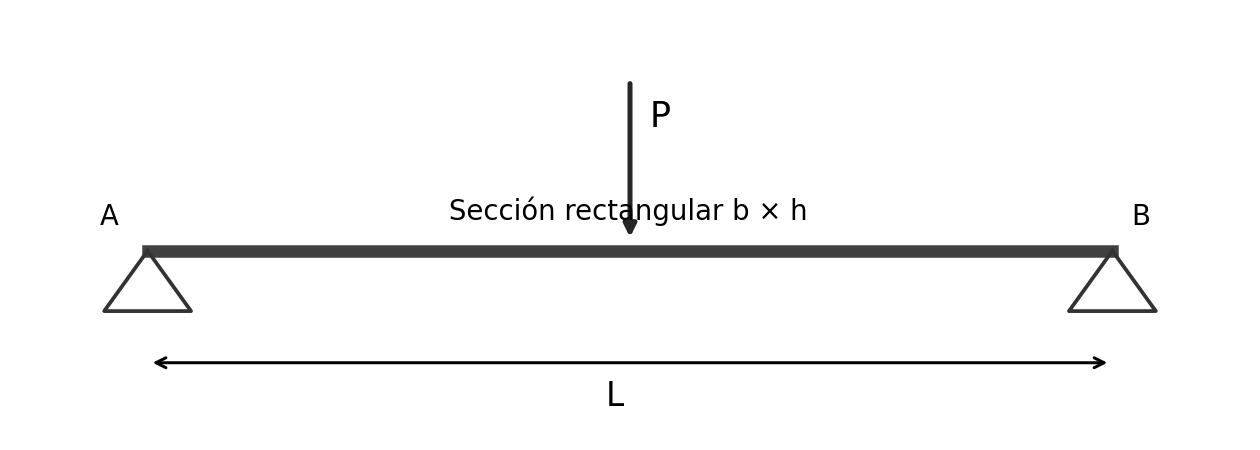
\includegraphics[width=0.69\linewidth]{esquema_viga.png}
\caption{Configuración del caso. Esquema original proporcionado en la actividad.}
\end{figure}

Se considera $h$ en la dirección de la flexión, sección y módulo constantes, apoyos ideales sin desplazamiento vertical y pequeñas deformaciones. Se trabaja con magnitudes positivas de carga y deflexión. El modelo representa la respuesta incremental a $P$: no se añade peso propio, cuya información no fue proporcionada, y se omite la deformación por cortante.

\section{Método y unidades}
Para la sección rectangular y la configuración indicada se emplean:
\begin{equation}
I=\frac{bh^3}{12}=\frac{0{,}20\,(0{,}40)^3}{12}
=\ensuremath{1{,}066666667\times10^{-3}\,\mathrm{m}^{4}},\qquad
\delta_{\mathrm{teo}}=\frac{PL^3}{48EI}.
\label{eq:modelo}
\end{equation}
La expresión de la deflexión central corresponde a flexión en tres puntos y coincide con las fuentes consultadas \cite{roylance2000,wierzbicki2013}. El cálculo utiliza $P\,[\mathrm{N}]=1000\,P\,[\mathrm{kN}]$, $E=25\times10^9\,\mathrm{N/m^2}$ y dimensiones en metros. La salida en metros se multiplica por 1000 para obtener milímetros. Así, $\delta_{\mathrm{teo}}[\mathrm{mm}]=0{,}05000\,P[\mathrm{kN}]$.

Se define $\Delta=\delta_{\mathrm{med}}-\delta_{\mathrm{teo}}$ y, para $P>0$, $e_r=100\,|\Delta|/|\delta_{\mathrm{teo}}|$. La referencia del porcentaje es la predicción teórica. Para $P=0$, el cociente no está definido y se registra ``n.a.''; el dato se mantiene en la figura.

\newpage
\section{Resultados y trazabilidad}
La Tabla~\ref{tab:resultados} reúne todas las cargas, sin descartar registros ni ajustar el módulo de elasticidad. La deflexión teórica aumenta \ensuremath{0{,}25\,\mathrm{mm}} por cada incremento de \ensuremath{5\,\mathrm{kN}}.

\begin{table}[H]
\centering
\caption{Comparación de las nueve observaciones. Los porcentajes se calculan antes de redondear.}
\label{tab:resultados}
\renewcommand{\arraystretch}{1.20}
\begin{tabular}{rrrrr}
\toprule
$P$ (kN) & $\delta_{\mathrm{med}}$ (mm) & $\delta_{\mathrm{teo}}$ (mm) & $\Delta$ (mm) & $e_r$ (\%) \\
\midrule
0  & 0,00 & 0,00 & 0,00 & n.a. \\
5  & 0,26 & 0,25 & 0,01 & 4,00 \\
10 & 0,50 & 0,50 & 0,00 & 0,00 \\
15 & 0,76 & 0,75 & 0,01 & 1,33 \\
20 & 1,01 & 1,00 & 0,01 & 1,00 \\
25 & 1,28 & 1,25 & 0,03 & 2,40 \\
30 & 1,54 & 1,50 & 0,04 & 2,67 \\
35 & 1,77 & 1,75 & 0,02 & 1,14 \\
40 & 2,05 & 2,00 & 0,05 & 2,50 \\
\bottomrule
\end{tabular}
\end{table}

\begin{figure}[H]
\centering
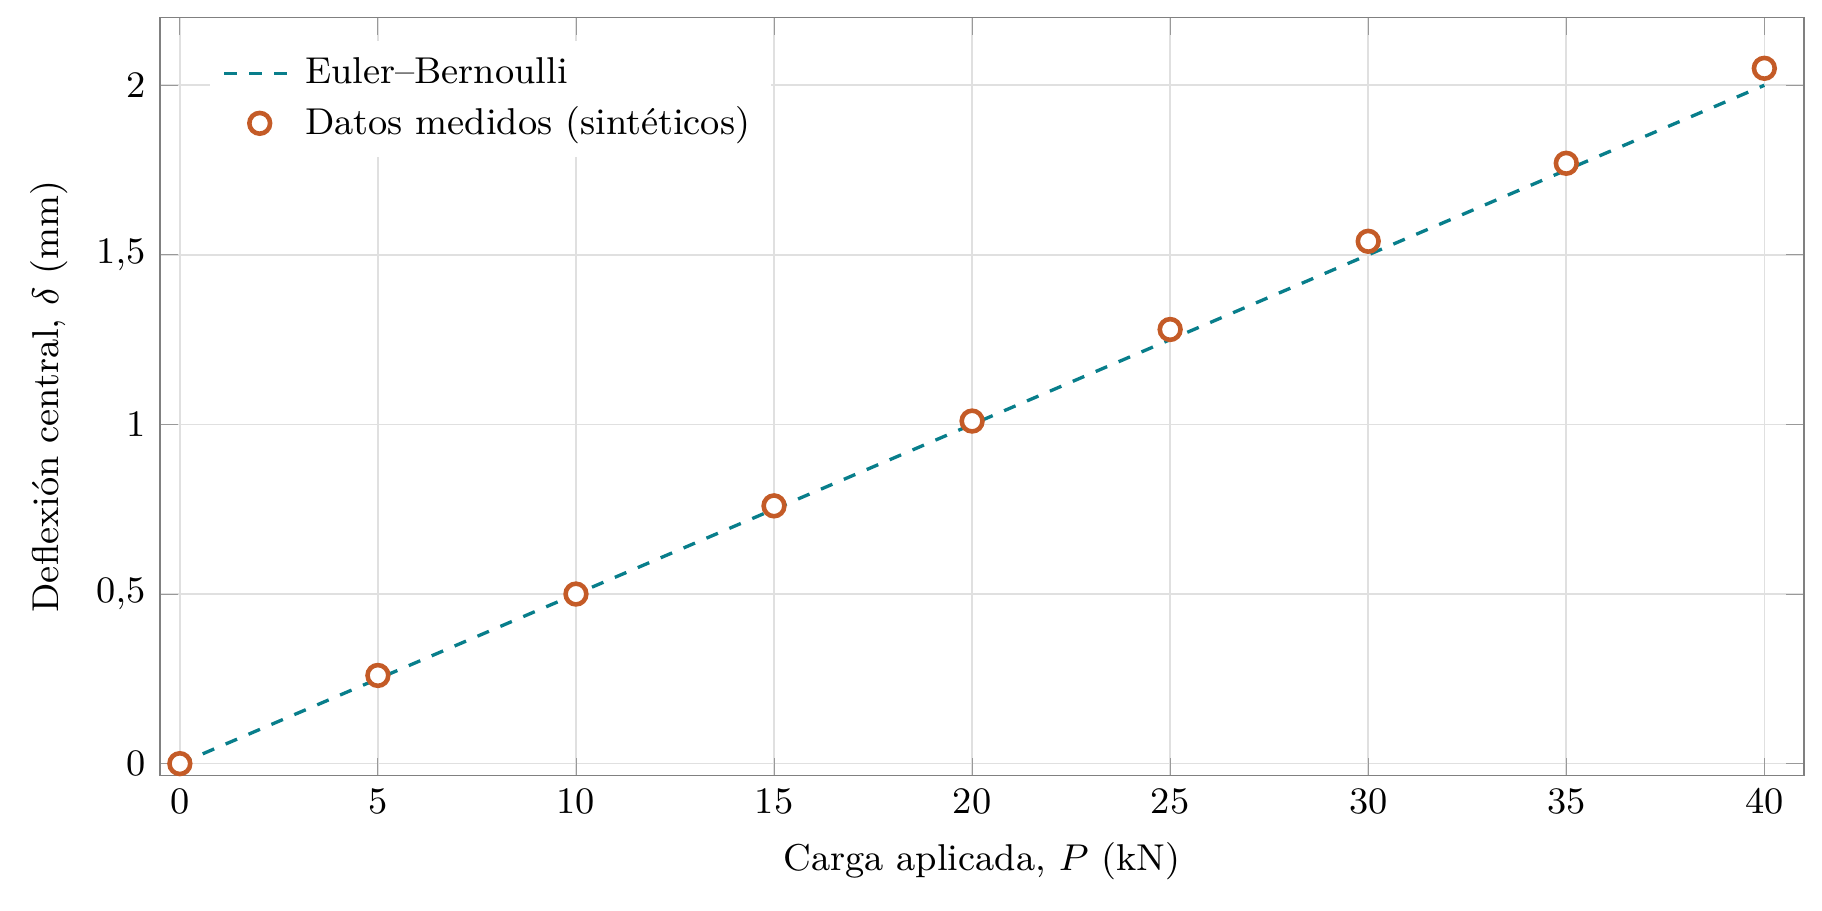
\includegraphics[width=0.95\linewidth]{carga_deflexion.png}
\caption{Comparación carga--deflexión. Los nueve puntos de cada serie proceden de \texttt{Analisis!B24:B32}, \texttt{D24:D32} y \texttt{F24:F32} de la planilla. La línea representa el modelo y los círculos, los datos sintéticos.}
\label{fig:curva}
\end{figure}

En las ocho cargas no nulas, $e_r$ varía entre \ensuremath{0{,}00\,\%} y \ensuremath{4{,}00\,\%}, con una media aritmética de \ensuremath{1{,}88\,\%}. La diferencia relativa mayor ocurre a \ensuremath{5\,\mathrm{kN}}, donde \ensuremath{0{,}01\,\mathrm{mm}} representa el \ensuremath{4\,\%} de la predicción. La diferencia absoluta máxima aparece a \ensuremath{40\,\mathrm{kN}}: \ensuremath{2{,}05\,\mathrm{mm}} medidos frente a \ensuremath{2{,}00\,\mathrm{mm}} teóricos, es decir, \ensuremath{0{,}05\,\mathrm{mm}} y \ensuremath{2{,}50\,\%}.

La planilla conserva una columna con la fila original del CSV. Las entradas se copian en la hoja \texttt{Datos}; las conversiones, fórmulas y comprobaciones se encuentran en \texttt{Analisis}. La figura publicada utiliza \texttt{analysis/datos\_figura.csv}, exportado de esas mismas celdas. El procedimiento de actualización se describe en el \texttt{README.md}.

\newpage
\section{Verificaciones e interpretación}
La revisión dimensional de la ecuación~\ref{eq:modelo} entrega una longitud:
\[
\frac{\mathrm{N}\,\mathrm{m}^3}{(\mathrm{N/m^2})\,\mathrm{m}^4}=\mathrm{m}.
\]
Como comprobación independiente se repitió el cálculo de la última carga en N y mm, convirtiendo nuevamente los parámetros originales:
\[
L=4000\,\mathrm{mm},\quad b=200\,\mathrm{mm},\quad h=400\,\mathrm{mm},\quad E=25000\,\mathrm{N/mm^2},
\]
\[
I=\frac{200\,(400)^3}{12}=\ensuremath{1{,}066666667\times10^{9}}\,\mathrm{mm^4},\qquad
\delta=\frac{40000\,(4000)^3}{48\,(25000)\,(200\,(400)^3/12)}=\ensuremath{2{,}000\,\mathrm{mm}}.
\]
El resultado coincide con la fila de \ensuremath{40\,\mathrm{kN}}. Además, para $P>0$, $\delta_{\mathrm{med}}/P$ se encuentra entre \ensuremath{0{,}05000} y \ensuremath{0{,}05200\,\mathrm{mm/kN}}, con promedio \ensuremath{0{,}05094\,\mathrm{mm/kN}}; el modelo entrega \ensuremath{0{,}05000\,\mathrm{mm/kN}} constante. Esta variación acotada es compatible con una respuesta aproximadamente proporcional en el intervalo analizado.

Siete de las ocho observaciones no nulas superan levemente la predicción y una coincide con ella. Se observa, por tanto, una pequeña tendencia hacia deflexiones mayores. Como no se dispone de incertidumbres ni repeticiones y los datos son sintéticos, no se puede atribuir esa diferencia a instrumentos, fisuración, apoyos o propiedades reales del material. Tampoco se establece un umbral normativo de aceptación a partir del \ensuremath{4\,\%} observado.

\section{Limitaciones y conclusiones}
La teoría adoptada no incorpora deformación por cortante, pérdida de rigidez, fluencia ni comportamiento no lineal. La relación $L/h=10$ hace pertinente revisar la hipótesis de despreciar cortante en un estudio más detallado, pero no se dispone del módulo de corte para cuantificar su aporte. La deflexión medida máxima equivale al \ensuremath{0{,}05125\,\%} de la luz; su pequeña magnitud es compatible con pequeñas deformaciones, sin demostrar por sí sola todas las hipótesis del modelo.

Para las cargas proporcionadas, el modelo reproduce de forma cercana la tendencia de los datos: el segundo momento de área es \ensuremath{1{,}06667\times10^{-3}\,\mathrm{m}^{4}}, la deflexión teórica máxima es \ensuremath{2{,}00\,\mathrm{mm}} y la diferencia relativa media es \ensuremath{1{,}88\,\%}. Las comprobaciones dimensional, numérica y de proporcionalidad apoyan la coherencia del cálculo. Estas conclusiones se limitan al ejercicio docente y al rango de 0 a \ensuremath{40\,\mathrm{kN}}.

\section{Reproducibilidad y asistencia de IA}
El proyecto distingue originales en \texttt{data/}, cálculos en \texttt{analysis/}, la figura en \texttt{figures/} y las fuentes LaTeX, BibTeX y PDF en \texttt{report/}. El análisis se puede continuar con Excel y Overleaf. La URL y el hash de la versión publicada se registran en la entrega de Moodle.

Se utilizó ChatGPT (Codex) para apoyar las fórmulas, la organización y la comunicación. Se contrastaron las ecuaciones con las fuentes citadas, se cotejaron las nueve filas y se verificó una carga en N y mm. El contenido incorporado y las comprobaciones se registran en \texttt{USO\_IA.md}. La IA no se utiliza como fuente técnica.

\small
\setlength{\parskip}{2pt}
\bibliographystyle{unsrt}
\IfFileExists{report/referencias.bib}{\bibliography{report/referencias}}{\bibliography{referencias}}
\end{document}
